\subsection{Υπολογισμός μεταφοράς βάρους}

Όταν το όχημα επιταχύνει, δημιουργούνται αδρανειακά φορτία στο κέντρο μάζας του
οχήματος. Καθώς το κέντρο μάζας βρίσκεται πάνω από το επίπεδο του δρόμου, δημιουργείται
ροπή που αντιδράται στα κατακόρυφα φορτία των τροχών. Αυτό το φαινόμενο ονομάζεται 
\emph{μεταφορά βάρους} και εξηγεί γιατί σε στροφές φορτίζονται οι εξωτερικοί τροχοί,
ή σε φρενάρισμα οι εμπρόσθιοι τροχοί.\\[10pt]
\noindent
Με βάση τις απλοποιήσεις του μοντέλου που θεωρούν το αμάξωμα ως άκαμπτο, αμελούμε τις
ελαστικές μεταφορές βάρους και την κλίση του αμαξώματος επάνω στις αναρτήσεις. ακολουθώντας
τα διαγράμματα ελευθέρου σώματος που περιγράφονται στα 
\cref{fig:longitudinalWeightTransfer,fig:lateralWeightTransfer}, προκύπτουν οι 
\cref{eq:longitudinalWeightTransfer,eq:lateralWeightTransfer} από ισορροπία ροπών.


\begin{equation}
    WF_{z,\text{long}} = \dfrac{Ma_xh}{L}
    \label{eq:longitudinalWeightTransfer}
\end{equation}

\begin{equation}
    WF_{z,\text{lat}} = \dfrac{Ma_yh}{t_{avg}}
    \label{eq:lateralWeightTransfer}
\end{equation}

Όπου,

\begin{itemize}
    \item $h$, το ύψος του κέντρου μάζας,
    \item $L$, το μεταξόνιο,
    \item $t_{avg} = \dfrac{t_f+t_r}{2}$, ο μέσος όρος των μετατροχίων του εμπρόσθιου και οπίσθιου άξονα,
    \item $\alpha_x = \dfrac{\Sigma F_x}{M}$, η διαμήκης επιτάχυνση του οχήματος,
    \item $\alpha_y = \dfrac{\Sigma F_y}{M}$, η εγκάρσια επιτάχυνση του οχήματος.
\end{itemize}

\begin{figure}[ht!]
    \begin{center}
        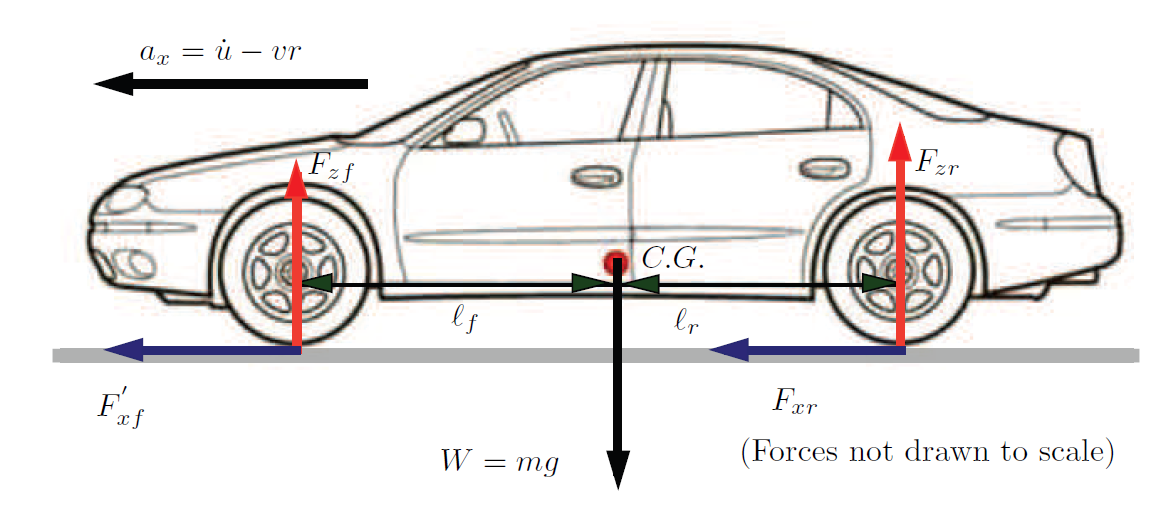
\includegraphics[width=0.7\textwidth]{figures/longitudinal-weight-transfer.png}
    \end{center}
    \caption{Διάγραμμα ελευθέρου σώματος -- διαμήκης μεταφορά βάρους \cite{tsiotras}.}
\label{fig:longitudinalWeightTransfer}.
\end{figure}

\begin{figure}[ht!]
    \begin{center}
        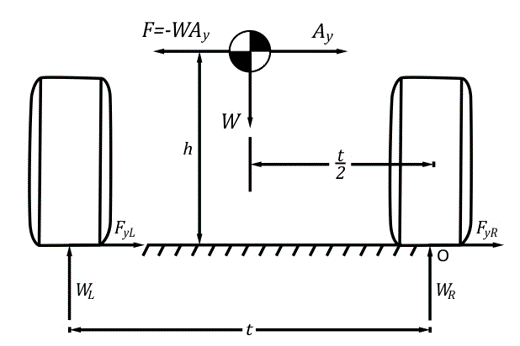
\includegraphics[width=0.6\textwidth]{figures/lateral-weight-transfer.png}
    \end{center}
    \caption{Διάγραμμα ελευθέρου σώματος -- εγκάρσια μεταφορά βάρους.}
\label{fig:lateralWeightTransfer}.
\end{figure}

\subsection{Υπολογισμός κατακόρυφου φορτίου τροχών}

Με βάση τις σχέσεις που αναπτύχθηκαν παραπάνω, τα κατακόρυφα φορτία σε κάθε τροχό παρατίθενται
στις σχέσεις \ref{eq:normalLoads}.

\begin{equation}
   F_{z,static,f} = MgWD
   \label{eq:staticFrontWeight} 
\end{equation}

\begin{equation}
   F_{z,static,r} = Mg(1-WD)
   \label{eq:staticRearWeight} 
\end{equation}

\begin{equation}
    \begin{aligned}
       F_{z,FL} &= F_{z,static,f} -\dfrac{WT_{long}}{2} - D_{roll}WT_{lat} + \dfrac{F_{z,f,lift}}{2}\\[10pt]
       F_{z,FR} &= F_{z,static,f} -\dfrac{WT_{long}}{2} + D_{roll}WT_{lat} + \dfrac{F_{z,f,lift}}{2}\\[10pt]
       F_{z,RL} &= F_{z,static,r} +\dfrac{WT_{long}}{2} - (1-D_{roll})WT_{lat} + \dfrac{F_{z,r,lift}}{2}\\[10pt]
       F_{z,RR} &= F_{z,static,r} +\dfrac{WT_{long}}{2} + (1-D_{roll})WT_{lat} + \dfrac{F_{z,r,lift}}{2}
    \end{aligned}
    \label{eq:normalLoads}
\end{equation}

Σημειώνεται η χρήση της παραμέτρου $D_{roll} \in [0,1]$ που μοιράζει την εγκάρσια μεταφορά βάρους στον
εμπρός και πίσω άξονα. Στην πραγματικότητα, η εγκάρσια μεταφορά βάρους δεν ισομοιράζεται στους δύο άξονες, αλλά επηρεάζεται έντονα
από την κατανομή βάρους και τη σχετική δυσκαμψία του κάθε άξονα. Η κατανομή αυτή επηρεάζει σε μεγάλο βαθμό 
και την υποστροφική / υπερστροφική συμπεριφορά του οχήματος, οπότε ακόμη και με απλή μοντελοποίηση του οχήματος ως άκαμπτο, αξίζει η συμπερίληψη αυτού του φαινομένου.